\documentclass{article}
\usepackage{tikz}
\usepackage{siunitx}
\usepackage{amsmath}

\begin{document}

\begin{figure}[h]
    \centering
    \begin{tikzpicture}[scale=2]
        % Draw the Ewald sphere
        \draw[blue, thick] (0,0) circle (1);
        
        % Draw the axes
        \draw[->] (-1.2,0) -- (1.2,0) node[right] {$k$};
        \draw[->] (0,-0.2) -- (0,1.2) node[above] {$k_z$};
        
        % Draw the black curve (first Born approximation)
        \draw[thick, black] plot[domain=-180:0, samples=100] (\x,{sqrt(1-cos(\x r))});
        
        % Draw the red dot on the black curve
        \filldraw[red] (90:1) circle (1pt);
        
        % Draw the dashed line from the origin to the red dot
        \draw[dashed] (0,0) -- (90:1);
        
        % Draw the vertical line from the red dot to the x-axis
        \draw[dashed] (90:1) -- (90:1 |- 0,0);
        
        % Label points
        \node at (90:1) [left] {$(k,k_z)$};
        \node at (0,0) [below left] {$(0,0)$};
        \node at (0,1) [left] {$(0,k_z)$};
        \node at (90:1 |- 0,0) [below right] {$(k,0)$};
        
        % Draw the angle theta/2
        \draw[->] (0,0) -- (30:1) node[midway, above right] {$\theta/2$};
        
        % Draw the angle theta
        \draw[->] (0,0) -- (60:1) node[midway, above right] {$\theta$};
        
        % Draw the vector 1/lambda
        \draw[->] (0,0) -- (45:1) node[midway, above right] {$\frac{1}{\lambda}$};
        
        % Draw the vector 1/lambda
        \draw[->] (0,0) -- (135:1) node[midway, above left] {$\frac{1}{\lambda}$};
        
        % Draw the text for the caption
        \node at (0.5,0.5) [below right] {\textbf{Geometrical equivalence of the Ewald sphere curvature (blue) and the first Born approximation of the multislice formalism (black). The black curve represents the complex-valued exitwave, $\psi_{\mathrm{exit}}$, that is mapped onto a paraboloid in Fourier space (Eq.~\eqref{eq:equiv}). At a small angle, $\theta \approx \lambda k$, the surface of the paraboloid approaches that of the Ewald sphere since $k_z = \tan \frac{\theta}{2} \approx \frac{k\theta}{2} = \frac{\lambda k^2}{2}$. For example, for a \SI{200}{\keV} electron beam ($\lambda \approx \SI{0.025}{\angstrom}$) and $k = \SI{1}{\angstrom^{-1}}$, the angle is $\theta \approx \SI{0.025}{\radian}$.}};
    \end{tikzpicture}
    \caption{Geometrical equivalence of the Ewald sphere curvature (blue) and the first Born approximation of the multislice formalism (black). The black curve represents the complex-valued exitwave, $\psi_{\mathrm{exit}}$, that is mapped onto a paraboloid in Fourier space (Eq.~\eqref{eq:equiv}). At a small angle, $\theta \approx \lambda k$, the surface of the paraboloid approaches that of the Ewald sphere since $k_z = \tan \frac{\theta}{2} \approx \frac{k\theta}{2} = \frac{\lambda k^2}{2}$. For example, for a \SI{200}{\keV} electron beam ($\lambda \approx \SI{0.025}{\angstrom}$) and $k = \SI{1}{\angstrom^{-1}}$, the angle is $\theta \approx \SI{0.025}{\radian}$.}
    \label{fig:ewald_sphere}
\end{figure}

\end{document}